%\documentclass{scrartcl}
\documentclass[11pt,a4paper]{article}
%\KOMAoptions{%
%  fontsize=11pt,      % Tamaño de fuente
%  paper=A4,           % Tamaño del papel
%  titlepage=true,    % Reserva una página para el título.
  %twoside=true,       % Para imprimir a doble página
  %headings=normal,    % Tamaño de letra para los títulos: small, normal, big
  %parskip=half,       % Espacio entre párrafos: full (una línea) o half (media línea)
  %headsepline=false,  % Una linea separa la cabecera del texto
  %listof=totoc,      % Añadir a los contenidos la lista de tablas y figuras
  %bibliography=totoc,% Añadir a los contenidos una entrada para la bibliografía
  %bibliography=openstyle,  % oldstyle
  %draft              % Para versiones de revisión, muestra las líneas mal formateadas
%}

\usepackage[english,spanish, es-tabla]{babel}
\usepackage[top=1.5cm, left=2.5cm, right=2.5cm, bottom=2.5cm]{geometry}
\usepackage{mystyle}
\usepackage{mycolours}
\usepackage{mytcolorbox}
\usepackage{mycommands}
\usepackage{microtype}
\usepackage{pdflscape}
\usepackage{rotating}
\usepackage{epsfig} % para poner poner imágenes eps
\graphicspath{{images/}}
\UseTblrLibrary{siunitx}
\usepackage{microtype}
\usepackage{chemfig}
\usepackage{schemata}
%\usepackage{xymtex}

%%%%%%%%%%%%%%%%%%%%%%%%%%%%%%%%%%%%%
% Encabezado y pie de página
%%%%%%%%%%%%%%%%%%%%%%%%%%%%%%%%%%%%%%

% \usepackage{fancyhdr}
% \pagestyle{fancy}
% \lhead{Formulación Orgánica}
% \rhead{IES José Conde García (Almansa)}

\usepackage{lastpage} %Se necesita para la última página.
\usepackage{fancyhdr}
    \setlength{\headheight}{43.00pt}
    \pagestyle{fancy}
    \fancyhf{}
    \chead{\negrita{Formulación Orgánica}\vspace*{0.3pt}}
    \rhead{
\includegraphics[scale=0.07]{logos/logo_Conde.jpeg}}
    \lhead{Dpto. Física y Química\vspace*{0.3pt}}
    %\cfoot{Página \azuln{\thepage}\ de \azuln{\pageref{LastPage}}}
    \cfoot{\azuln{\thepage}\ de \azuln{\pageref{LastPage}}}


\setchemfig{atom sep=2.1em}
\title{\huge \bfseries \sffamily Formulación Química Orgánica}
\author{\Large \bfseries \sffamily IES José Conde García\\\bfseries \sffamily Almansa (Albacete)}
\date{}
\usepackage{soulutf8} %usar en lugar de soul para los acentos  pasado a mi estilo general
%%%%%%%%%%%%%%%%%%%%%%%%%%%%%%%%%%%%%%%%%%%%%%%%%%%%%%%%%%%%%%%%%%%%%%
% COMANDOS
%%%%%%%%%%%%%%%%%%%%%%%%%%%%%%%%%%%%%%%%%%%%%%%%%%%%%%%%%%%%%%%%%%%%%%
\usepackage{titlesec}

\titleformat{\section}
    {\normalfont\Large\sffamily\bfseries\color{darkblue}}
    {\tcbox[colback=darkblue, colframe=darkblue, coltext=blue!1, on line, boxsep=0pt, left=4pt, right=4pt, top=4pt, bottom=4pt]{\thesection}}{0.5em}{}


\titleformat{\subsection}
    {\normalfont\large\sffamily\bfseries\color{darkblue!80}}
    {\hspace{2mm}\tcbox[colback=darkblue!70, colframe=darkblue, coltext=blue!1, on line, boxsep=0pt, left=4pt, right=4pt, top=4pt, bottom=4pt]{\thesubsection}}{0.5em}{}


\DeclareCaptionFont{blue}{\color{blue254}} % es necesario declarar el color para que función
\captionsetup{labelfont={blue,bf}}
%\usepackage[hang,flushmargin]{footmisc} % para que en las notas al pie no me idente el párrafo. ller paquete.
\newcommand{\mybox}[1]{\xmybox{\phantom{l}\textbf{#1}\phantom{j}}}
\newcommand{\marcador}[1]{\colorbox{yellow}{#1}}

\newcommand{\caja}[1]{\begin{center}%
                    \begin{impt}%
                        #1
                    \end{impt}
                    \end{center}}
    

\definesubmol{aldehido}{C(=[2]O)(-[0]H)} 
\definesubmol{aldehido2}{H-C(=[2]O)} 
\definesubmol{fenil}{**6(------)}
\definesubmol{ciclopentil}{*5(-----)}
\definesubmol{ciclohexil}{*6(------)}
\definesubmol{acido}{C(=[2]O)(-[0]OH)}
\definesubmol{acido2}{C(-[4]HO)(=[2]O)}


\UseTblrLibrary{varwidth}




\begin{document}
\spacing{1.3}
\maketitle
\tableofcontents


\newpage{}

\myemptypage{}

\newpage{}

\section{Introducción}



La \blueremark{química} \blueremark{orgánica} hace referencia a la química en la que sus compuestos están formados mayoritariamente por hidrógeno y carbono. A los elementos distintos al hidrógeno y carbono se les denomina \blueremark{heteroelementos} como por ejemplo el oxígeno, nitrógeno, azufre, fósforo \dots

\section{Características generales de la química del carbono}

\subsection{Tipos de enlace en el átomo de carbono}

\caja{El átomo de carbono puede formar hasta 4 enlaces covalentes con otros átomos (normalmente dos enlaces suelen ser con otro átomo de carbono).} 

Estos enlaces pueden ser:

\begin{enumerate}[label=\numberballmDarkTeal]
    \item \textbf{\azul{Enlaces sencilos}}: Los dos átomos comparten un par de electrones. A los compuestos con enlaces sencillos se les denomina \rojo{compuestos saturados}. La geometría de este tipo de enlaces es tetrahédrica y por tanto los 4 enlaces sencillos se disponen hacia los vértices de un tetraedro regular formando entre sí ángulos de \ang{109.5}.\\
          Cuando un átomo de carbono presenta enlace sencillo, se dice que el átomo de carbono tiene una hibridación \azul{$sp^3$}
          \begin{figure}[H]
              \centering
              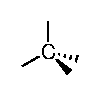
\includegraphics[scale=1.5]{enlace_sencillo.eps}
              \caption{Enlace sencillo. Hibridación $sp^3$}
              \label{fig:enlacesencillo}
          \end{figure}
    \item \textbf{\azul{Enlaces dobles}}: Los dos átomos comparten dos pares de electrones. El enlace doble y los enlaces sencillos forman ángulos de \ang{120} localizándose en un plano.

          \begin{figure}[H]
              \centering
              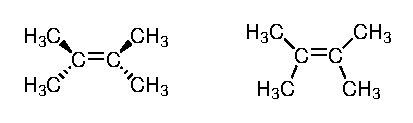
\includegraphics[scale=1]{dobleenlace.eps}
              \caption{Enlace doble. Hibridación $sp^2$}
              \label{fig:enlacedoble}
          \end{figure}


          Cuando un átomo de carbono presenta enlace doble, se dice que el átomo de carbono tiene una hibridación \azul{$sp^2$}
    \item \textbf{\azul{Enlaces triples}}: Los dos átomos comparten tres pares de electrones. El triple enlace y el enlace restante forman una línea recta (ángulo de \ang{180}).

          \begin{figure}[H]
              \centering
              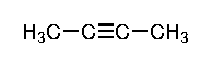
\includegraphics[scale=1]{enlacetriple.eps}
              \caption{Enlace triple. Hibridación $sp$}
              \label{fig:enlacetriple}
          \end{figure}

          Cuando un átomo de carbono presenta enlace doble, se dice que el átomo de carbono tiene una hibridación \azul{$sp$}

\end{enumerate}

\caja{A los compuestos que contienen enlaces simples se les denomina \blueremark{saturados} y aquellos compuestos que contienen dobles o triples enlaces se les denominan \blueremark{insaturados}}


\subsection{Representación de las moléculas orgánicas}

Existen principalmente 3 tipos o formas de representar moléculas orgánicas que son:

\begin{enumerate}[label=\numberballmDarkTeal]
    \item \textbf{\azul{Fórmula desarrollada}}: Se obtiene proyectando sobre el papel los distintos átomos que constituyen la molécula con sus correspondientes enlaces es decir, se escriben todos los enlaces y todos los átomos

          \begin{figure}[H]
              \centering
              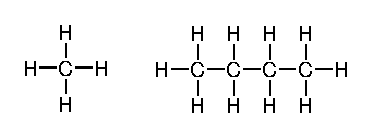
\includegraphics[scale=1]{desarrollada.eps}
              \caption{Fórmula desarrollada}
              \label{fig:formuladesarrollada}
          \end{figure}

    \item \textbf{\azul{Fórmula semidesarrollada}}: Es una de las más utilizadas y solamente se muestran los enlaces carbono-carbono.
          \begin{figure}[H]
              \centering
              \ch{CH_3-CH_2-CH=CH_2}
              \caption{Fórmula semidesarrollada}
              \label{fig:formulasemidesarrollada}
          \end{figure}

    \item \textbf{\azul{Fórmula simplificada}}: Es la más utilizada en química orgánica. En esta fórmula se omiten los átomos de carbono así como los átomos de hidrógeno quedando representados los enlaces carbono-carbono así como los enlaces carbono-heteroelemento. Cada punto de unión entre dos líneas (vértices) representa un átomo de carbono.
          \begin{figure}[H]
              \centering
              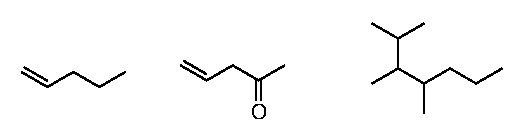
\includegraphics[scale=1]{simplificada.eps}
              \caption{Fórmula simplificada}
              \label{fig:formulasimplificada}
          \end{figure}
\end{enumerate}

\subsection{Grupo funcional y jerarquía}

Denominamos \blueremark{grupo funcional} al átomo o conjunto de átomos que caracterizan a una serie de compuestos orgánicos con propiedades y estructuras químicas similares.

Cuando tenemos varios grupos funcionales en una misma molécula, es necesario determinar el grupo funcional principal, el cual le dará el nombre quedando el resto como sustituyentes. En la siguiente tabla, se muestra la jerarquía ordenados de mayor a menor prioridad junto con la terminación si es grupo funcional así como la terminación si es un sustituyente:

\begin{table}[H]
    \centering
    \caption{Grupos funcionales como cadena principal y como sustituyente}
    \label{table:gruposfuncionales2}
    \begin{tblr}{
            colspec = { Q[c,m] | Q[c,m] | Q[c,m] | Q[c,m]},
            row{odd} = {bg=myOrange3!10},
            row{1} = {bg=myOrange3!90,fg=white,font=\bfseries}
        }
        \hline
        {Grupo\\ Funcional} & Fórmula & Principal & Sustituyente \\
        \hline
        Ac. Carboxílicos &\ch{R-COOH} & Ácido \dots --oico &  Carboxi-- \\
        Ac. Sulfónicos* &\ch{R-SO3H} &Ácido \dots --sulfónico &  Sulfo-- \\
        Anhídridos de ácido* &\ch{R-CO-O-CO-R'} & Anhídrido \dots --oico&  --\\
        Esteres & \ch{R-CO-O-R'} & {--ato\\carborxilato} & \dots oiloxi-- \\
        Haluros de ácido* &\ch{R-CO-X} & Halogenuro de \dots & Halocarbonil--\\
        Amidas & \ch{R-CO-NH2}& --amida & amido--\\
        Nitrilos  &\ch{R-CN} & --nitrilo & ciano-- \\
        Aldehídos &\ch{R-CO-H} & --al & {oxo-- \\ Formil--}\\
        Cetonas &\ch{R-CO-R'} & --ona & oxo--\\
        Alcoholes &\ch{R-OH} & --ol & hidroxi--\\
        Fenoles &\ch{Ar-OH} & --fenol & hidroxi--\\
        Tioles* & \ch{R-SH}& --tiol & mercapto-- \\
        Aminas & \ch{R-NH2}& --amina & amino--\\
        Iminas* &\ch{R-C=N-R'} & --imina & imino--\\
        Alquenos &\ch{R_{2}C=CR_{2}} & --eno & enil-- \\
        Alquinos &\ch{R-C+C-R} & --ino & inil--\\
        Alcanos &\ch{R-H} & --ano& il--\\
        \hline
        \SetCell[c=4]{l,bg=white}  * No los veremos en este curso
    \end{tblr}
\end{table}


\subsection{Serie homóloga}

Es el conjunto de compuestos que tienen el mismo grupo funcional y por tanto diferirán en el número de átomos de carbono así como la posición del grupo funcional.

Para indicar el número de átomos de carbono que forman la cadena carbonada de las diferentes series homólogas se utilizan los prefijos griegos como los de la siguiente tabla:
\begin{table}[H]
    \centering
    \caption{Serie homóloga}
    \label{table:seriehomologa}
    \begin{tblr}{
            colspec = {Q[c,m] | Q[c,m] | Q[c,m] | Q[c,m]},
            hlines = {1pt, solid},
            row{odd} = {bg=myOrange3!10},
            row{1} = {bg=myOrange3!90,fg=white,font=\bfseries}
        }
        {Número \\de carbonos} & Prefijo & {Número \\de carbonos} & Prefijo\\
        1 & Met-- & 11  & Undec-- \\
        2 & Et-- & 12 & Dodec-- \\
        3 & Prop-- &1 3 & Tridec--\\
        4 & But-- & 14 & Tetradec--\\
        5 & Pent-- & 15 & Pentadec--\\
        6 & Hex-- & 20 & Eicos--\\
        7 & Hept-- & 30 & Triacont-- \\
        8 & Oct-- & 40 & Tetracont--\\
        9 & Non-- & 50 & Pentacont--\\
        10 & Dec-- & 100 & Hecta--
    \end{tblr}
\end{table}


\section{Normas generales de formulación}

\begin{enumerate}[label=\numberballmDarkTeal]
    \item \azul{Determinar cadena principal}: Será la cadena que mayor número de átomos de carbono tenga.
          \begin{enumerate}
              \item Si existen más de dos cadenas con el mismo número de átomos de carbono, se toma como referencia aquella en la que el grupo funcional principal o los localizadores (sus posiciones) de los sustituyentes tengan los números más bajos (ver más adelante).
                    \begin{figure}[H]
                        \centering
                        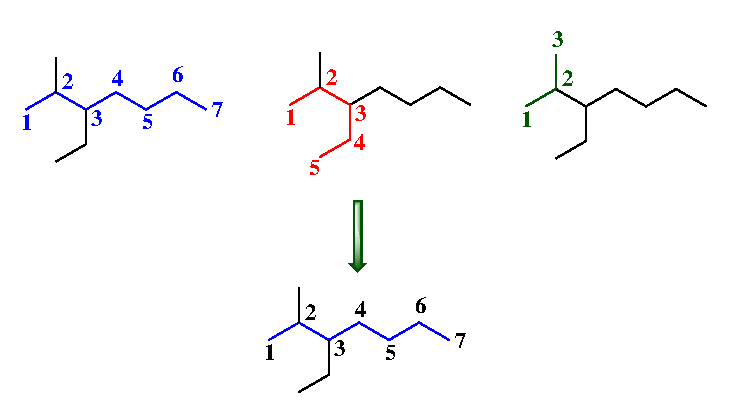
\includegraphics[scale=1]{cadenaprincipal.eps}
                        \caption{Elección de la cadena principal}
                        \label{fig:cadenaprincipal}
                    \end{figure}
              \item La cadena seleccionada en \textit{a)} será un \blueremark{heptano}
          \end{enumerate}

    \item Las cadenas o grupos unidos a la cadena principal se les denomina \blueremark{sustituyentes} o \blueremark{radicales}.
    \item Los radicales se ordenan alfabéticamente asignándoles un número como localizador que nos indica su posición.
    \item Los localizadores (números) se separan por comas.
    \item Los localizadores y las letras se separan por (--).
    \item De manera general, la nomenclatura de cualquier compuesto orgánico tendrá la siguiente forma:

          Sustituyentes + serie homóloga (indica número de carbonos) + grupo funcional no principal + grupo funcional principal
\end{enumerate}

\section{Grupos Funcionales}

\subsection{Hidrocarburos}

Son compuestos constituidos exclusivamente por carbono e hidrógeno y según el tipo de cadena se pueden clasificar en:\vspace{6pt}
\newpage

\begin{paracol}{2}
    \schema{
        \schemabox{Alifáticos}
    }
    {
        \schema{
            \schemabox{Lineales}
        }
        {
            \schemabox{Alcanos\\alquenos\\Alquinos}
        }
        \schema{
            \schemabox{Cíclicos}
        }
        {
            \schemabox{Cicloalcanos\\Cicloalquenos\\Cicloalquinos}
        }

    }

    \switchcolumn
    \vspace{10mm}
    \schema{
        \schemabox{Aromáticos}
    }
    {
        \schemabox{Monocícliclos\\Policíclicos}
    }
\end{paracol}

\subsubsection{Alcanos}

Corresponden a la fórmula general \ch{C_nH_{2n+2}}\vspace{6pt}

\mybox{Nomenclatura}

\begin{enumerate}[label=\numberballmDarkTeal]
    \item Se nombran con el prefijo indicativo de la serie homóloga (indica el número de átomos de carbono) seguido de la terminación \blueremark{-ano}\\
          \begin{figure}[H]
              \centering
              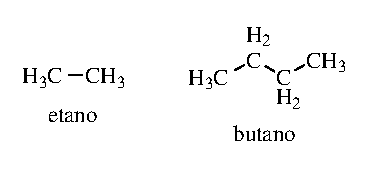
\includegraphics[scale=1]{alcanos1.eps}
          \end{figure}
    \item Si alguno de los alcanos pierde un átomo de hidrógeno se forma un \blueremark{radical alquílico}. A estos radicales se les considera \textbf{sustituyentes de la cadena principal}.
     Se nombran con la terminación \blueremark{-il} (si es un sustituyente) o \blueremark{-ilo} (si se nombra el radical)
          \begin{figure}[H]
              \centering
              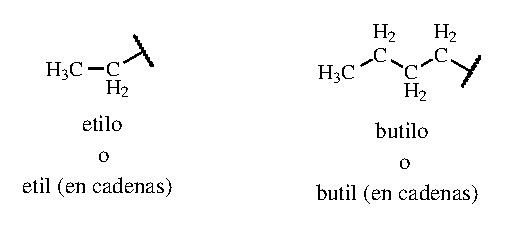
\includegraphics[scale=1]{alcanos2.eps}
          \end{figure}
    \item Existen radicales que tienen nombre propio admitido por la IUPAC:
          isopropil, n-butil, tercbutil, isobutil.
          \begin{figure}[H]
              \centering
              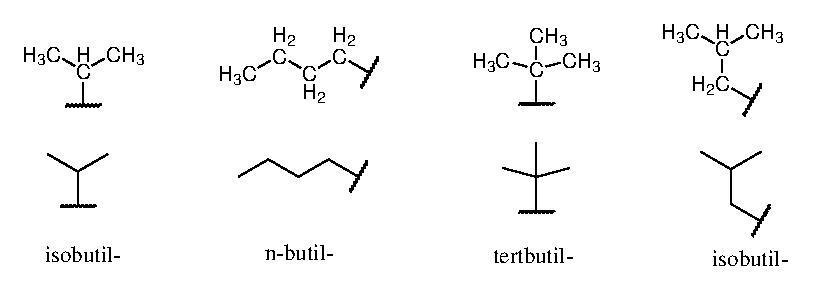
\includegraphics[scale=1]{alcanos3.eps}
          \end{figure}
    \item Si el alcano es ramificado, es decir tiene sustituyentes se siguen las siguientes reglas:
          \begin{enumerate}
              \item Se elige como cadena principal aquella que contenga mayor número de átomos de carbono. A continuación se numeran dichos átomos, de tal forma que las ramificaciones tengan los números localizadores más bajos.
              \item Se nombran primero la ramificación, con la terminación \blueremark{-il} indicando la posición donde se encuentra con un número.
              \item Si en la cadena principal hay dos radicales iguales se emplean los prefijos \textit{di-}, \textit{tri-}, \textit{tetra-} \dots anteponiendo los números que indican sus posiciones.
              \item Si en la cadena principal  hay dos o más ramificaciones, estas se nombran siguiendo el orden alfabético.
              \item Entre número y número se intercala con una coma.
              \item Entre número y letra se intercala con un guion.
              \item Nombramos la cadena principal.
              \item Si las ramificaciones son complejas, se nombran independientemente entre paréntesis.
          \end{enumerate}
          \begin{figure}[H]
              \centering
              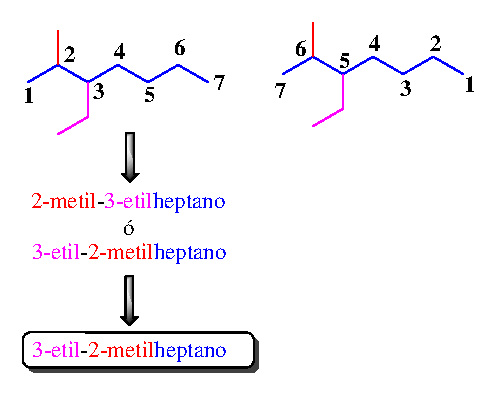
\includegraphics[scale=1]{alcanos4.eps}
          \end{figure}

          \begin{figure}[H]
              \centering
              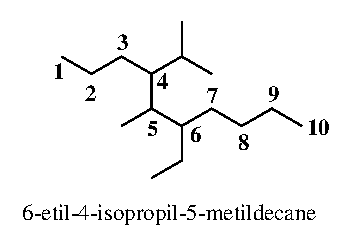
\includegraphics[scale=1]{alcanos5.eps}
          \end{figure}

\end{enumerate}


\subsubsection{Alquenos}

Presentan uno o más dobles enlaces carbonados (\chemfig{C=C}) y cuando tienen un único enlace tienen como formula general \ch{C_nH_{2n}}\vspace{6pt}

\mybox{\textbf{Nomenclatura}}

\begin{enumerate}[label=\numberballmDarkTeal]
    \item Los nombramos igual que los alcanos pero sustituyendo la terminación \blueremark{-ano} por la terminación \blueremark{-eno}.
    \item La posición del doble enlace se indica con un localizador que sea el menor posible.
    \item Si tenemos más de un doble enlace se emplea las terminaciones \blueremark{-dieno}, \blueremark{-trieno} \dots
    \item Al escribir el nombre, primero ponemos los radicales (si los tiene) con su  localizador (es la posición que ocupa el radical/sustituyente), luego el prefijo indicativo de la longitud principal (número de carbonos) y a continuación el localizador de los dobles enlaces con la terminación \blueremark{-eno}.
     \begin{figure}[H]
        \centering
        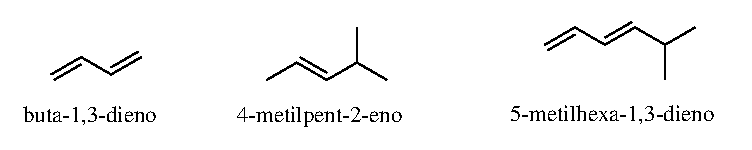
\includegraphics[scale=1]{alquenos1.eps}
    \end{figure}
    \item Cuando un alqueno actúa como radical, se utiliza la terminación \blueremark{-enil} o \blueremark{-enilo}
    \item Existen radicales que tienen nombre propio admitido por la IUPAC:
    \begin{figure}[H]
        \centering
        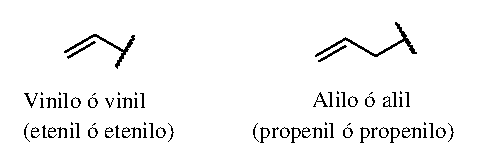
\includegraphics[scale=1]{alquenos2.eps}
    \end{figure}
\end{enumerate}



\subsubsection{Alquinos}

Son aquellos que presentan uno o más triples enlaces (\chemfig{C~C}) por lo que su fórmula general será \ch{C_nH_{2n-2}} si solo tenemos un único enlace.\vspace{6pt}

\mybox{\textbf{Nomenclatura}}

\begin{enumerate}[label=\numberballmDarkTeal]
    \item Sigue las mismas reglas que los alquenos pero utilizando la terminación \blueremark{-ino}
    \item con dobles y triples enlaces en la misma molécula por lo que las reglas a seguir para u nomenclatura serán:
          \begin{enumerate}
              \item La cadena principal es la que tiene mayor número de instauraciones (mayor número de dobles y triples enlaces) aunque exista una cadena más larga pero con menor número de insaturaciones.
              \item Una vez elegida la cadena principal, se empieza a numerar los carbonos por el extremo donde tengamos los localizadores más bajos para las insaturaciones.
              \item Si existiera varias cadenas con los mismos localizadores, se tomará en cuenta aquel en el que se le asigne el localizador más bajo al doble enlace.
              \item Se escriben primero los radicales con su correspondiente localizador + el prefijo que indica la longitud de la cadena principal + localizadores de los dobles y triples enlaces empezando por el alqueno.
              \item Si el alquino actúa como radical se emplea las terminaciones \blueremark{-inil} ó \blueremark{-enilo}
          \end{enumerate}
\end{enumerate}

\begin{figure}[H]
    \centering
    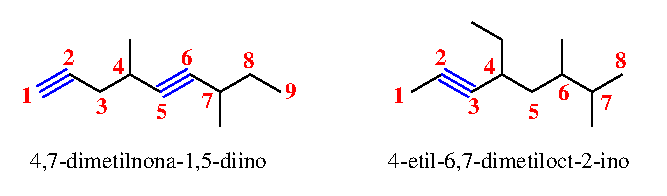
\includegraphics[scale=1]{alquinos1.eps}
\end{figure}

\begin{figure}[H]
    \centering
    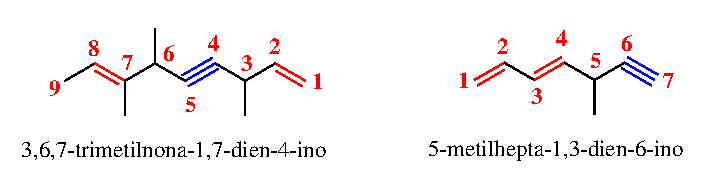
\includegraphics[scale=1]{alquinos2.eps}
\end{figure}


\subsection{Hidrocarburos cíclicos}

Son aquellos que forman un ciclo o un anillo, estos compuestos pueden provenir de alcanos, alquenos o alquinos, llamándose cicloalcanos, cicloalquenos o cicloalquinos respectivamente.\vspace{6pt}

\mybox{\textbf{Nomenclatura}}.

\begin{enumerate}[label=\numberballmDarkTeal]
    \item Se nombran como los correspondientes alcanos, alquenos o alquinos pero anteponiendo el prefijo \blueremark{ciclo-}
    \item Si tiene radicales  se nombran primero estos radicales con su correspondiente localizador.
    \item Se asignará el localizador más bajo según el orden alfabético de dichos radicales.
    \item En el caso de que el radical sea más complejo o más extensa que el propio ciclo, se nombra el hidrocarburo cíclico como un radical.

    \begin{figure}[H]
        \centering
        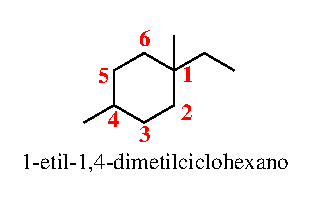
\includegraphics[scale=1]{hidrocarburosciclicos1.eps}
    \end{figure}

    \item En los \blueremark{cicloalquenos} y \blueremark{cicloalquinos} los carbonos se numeran de modo que los dobles y triples enlaces tengan los localizadores más pequeños.
    \item Si tenemos dobles y triples enlaces en la misma molécula, los dobles enlaces tienen prioridad frente a los triples enlaces para asignar el localizador.

    \begin{figure}[H]
        \centering
        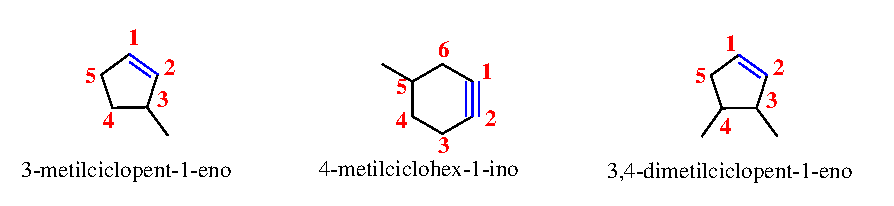
\includegraphics[scale=1]{hidrocarburosciclicos2.eps}
    \end{figure}
\end{enumerate}

\subsection{Hidrocarburo aromáticos}

Son aquellos hidrocarburos que derivan del benceno (\ch{C6H6}). El benceno un hidrocarburo cíclico de 6 átomos de carbono que posee tres enlaces sencillos y tres enlaces dobles, todos ellos deslocalizados es decir se van intercambiando.\vspace{6pt}

\mybox{Nomenclatura}

\begin{enumerate}[label=\numberballmDarkTeal]
    \item Se le nombra con el nombre de \blueremark{benceno}
    \begin{figure}[H]
        \centering
        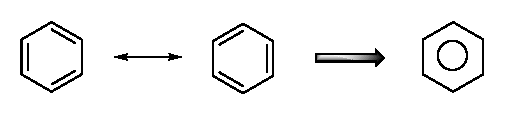
\includegraphics[scale=1]{benceno.eps}
    \end{figure}
    \item Si tiene radicales se nombran los radicales indicando el localizador y seguidamente el nombre de benceno.
    \item Si existen más de dos sustituyentes o radicales se indican la posición relativa de estos radicales con los números 1,2; 1,3; 1,4. Ordenando los sustituyentes por orden alfabético.
    \item En el caso de que haya más de dos sustituyentes, esto recibirán los localizadores más bajos y se nombrarán según su orden alfabético.
    \begin{figure}[H]
        \centering
        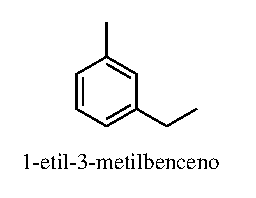
\includegraphics[scale=1]{aromaticos1.eps}
    \end{figure}
    \begin{figure}[H]
        \centering
        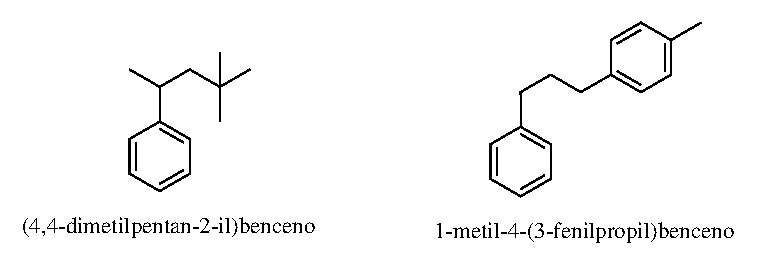
\includegraphics[scale=1]{aromaticos3.eps}
    \end{figure}
    \item Generalmente se suele utilizar los prefijos \blueremark{orto-}, \blueremark{meta-} y \blueremark{para-} para describir las posiciones 1,2; 1,3; 1,4 respectivamente.
    \begin{figure}[H]
        \centering
        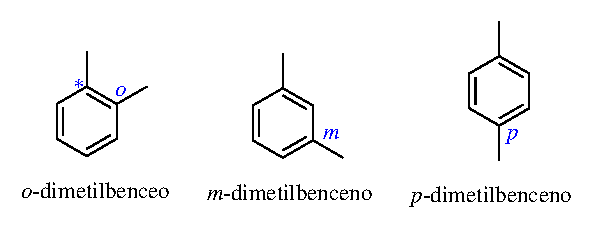
\includegraphics[scale=1]{aromaticos2.eps}
    \end{figure}
    \item Si el benceno actúa como radical en otra cadena carbonada, indica con el nombre de \blueremark{fenil} con el correspondiente localizador.
    
    \item Si un compuesto aromático tiene dos o más anillos de benceno no sustituidos, estos actuarán esn este caso como sustituyentes.
    \begin{figure}[H]
        \centering
        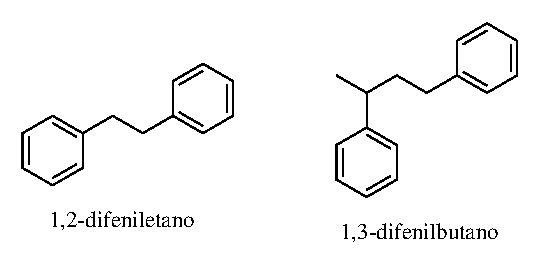
\includegraphics[scale=1]{aromaticos4.eps}
    \end{figure}
    
\end{enumerate}

\mybox{\textbf{Hidrocarburos aromáticos policíclicos}}

Existen hidrocarburos aromáticos con más de un anillo que a su vez los podemos dividir en:

\begin{enumerate}[label=\numberballmDarkTeal]
    \item \azul{\textbf{Anillos Aromáticos Policíclidos}}: Anillos de benceno unidos mediante un enlace sencillo.
          \begin{figure}[H]
              \centering
              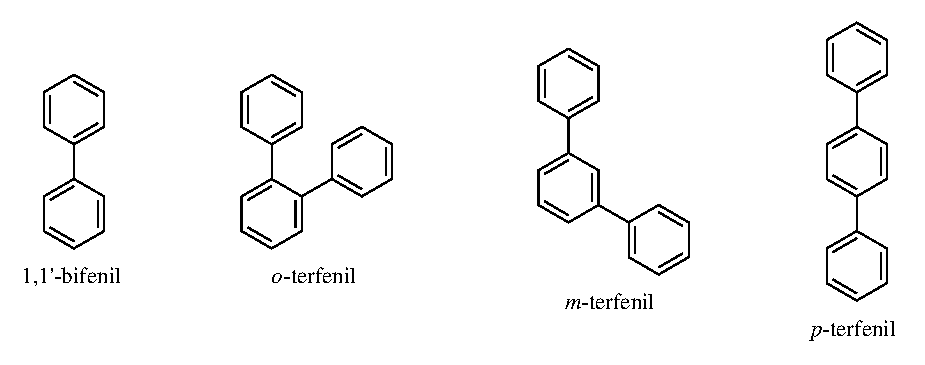
\includegraphics[scale=1]{aromaticospoliciclicos.eps}
              \caption{Anillos Aromáticos Policíclicos}
              \label{fig:aromaticospoliciclicos}
          \end{figure}
    \item \azul{\textbf{Anillos Condensados}}: Son aquellos compuestos en los que los anillos se encuentran condensados, siendo los más importantes:
          \begin{figure}[H]
              \centering
              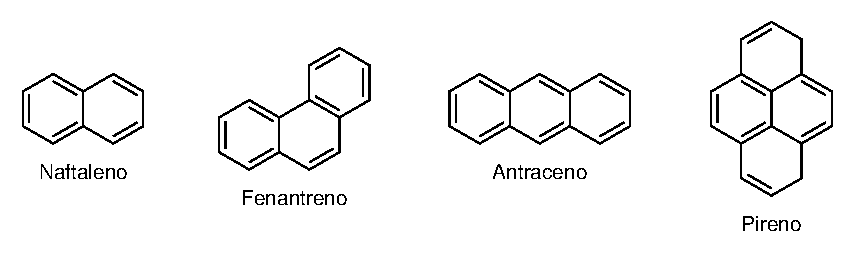
\includegraphics[scale=1]{condensados.eps}
              \caption{Anillos Aromáticos Condensados}
              \label{fig:aromaticoscondensados}
          \end{figure}
\end{enumerate}

\subsection{Derivados Halogenados}
Son compuestos obtenidos por la sustitución de uno o más hidrógenos por uno o más halógenos. Los más habituales son los halogenuros de alquilo es decir aquellos en los que se ha sustituido un halógeno por un hidrógeno en un alcano.

En este tipo de compuestos el grupo funcional será el halógeno y normalmente se representa con \blueremark{-X}.\vspace{6pt}

\mybox{\textbf{Nomenclatura}}

\begin{enumerate}[label=\numberballmDarkTeal]
    \item Se nombran anteponiendo al nombre del hidrocarburo el nombre del halógeno.
    \item Si tenemos más de un halógeno se numeran siempre con los localizadores más bajos posibles.
    \item Si un mismo halógeno aparece varias veces, se utilizan los prefijos \blueremark{di-}, \blueremark{tri-} \dots
          \begin{figure}[H]
              \centering
              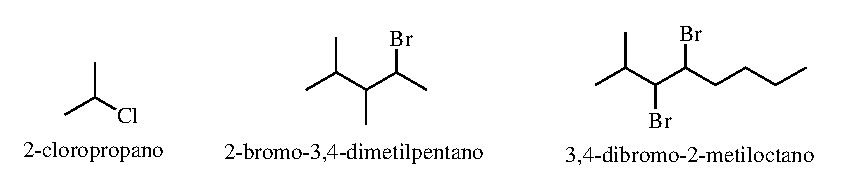
\includegraphics[scale=1]{halogenuros1.eps}
          \end{figure}
\end{enumerate}

\subsection{Alcoholes}

Son compuestos derivados de los hidrocarburos, en los que se ha sustituido un hidrógeno por un grupo \ch{-OH}.\vspace{6pt}

\mybox{\textbf{Nomenclatura}}

\begin{enumerate}[label=\numberballmDarkTeal]
    \item Se nombran como los alcanos de los que proceden quitando \blueremark{-o} de la terminación \blueremark{-ano} y añadiendo la terminación \blueremark{-ol}. Se debe indicar la posición con en la que se encuentra el grupo \ch{-OH} con un localizador lo más bajo posible.
    \item Si en la molécula hay más de un grupo \ch{-OH}, se utilizan los prefijos \blueremark{di-}, \blueremark{tri-} \dots indicando con localizadores las posiciones en las que se encuentran. Estos prefijos quedarían por tanto como \blueremark{diol-}, \blueremark{triol-}, \blueremark{tetraol-}\dots
    \item Para empezar a numerar, se elige la cadena que contenta el localizador más bajo para el grupo \ch{-OH}
    \item Si en la misma molécula hubiera insaturaciones (dobles o triples enlaces) el grupo \ch{-OH} tiene preferencia con respecto a esas insaturaciones para determinar la cadena principal.
    \item Como siempre, se escriben primero los radicales con su localizador, luego el prefijo que indica la longitud de la cadena principal, a continuación las insaturaciones, es decir los dobles y triples enlaces si los hubiera y luego la localización y el número de grupos \ch{-OH}
    \item Si un grupo \ch{-OH} actuara como radical, este se nombraría como \blueremark{hidroxi-}
\end{enumerate}

\begin{figure}[H]
    \centering
    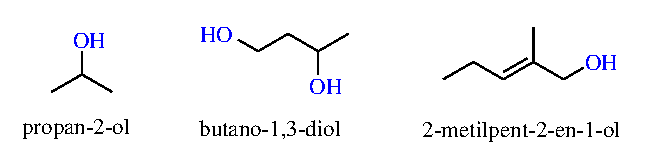
\includegraphics[scale=1]{alcoholes1.eps}
\end{figure}


\subsection{Éteres}

Son compuestos que resultan de la unión de dos radicales alquilo o arilo (proviene del anillo de benceno) mediante un puente de oxígeno según la siguiente estructura general, siento R y R' los radiales alquilo o arilo: \chemfig{R-O-R'}.\vspace{6pt}

\mybox{Nomenclatura}

\begin{enumerate}[label=\numberballmDarkTeal]
    \item Se nombran los dos radicales R y R' por orden alfabético seguido de la palabra \blueremark{éter}.
    \item Si ambos radicales son identicos se nombran anteponiendo el prefijo \blueremark{di-}
    \item Otra forma alternativa de nombrar los éteres será:
          \begin{enumerate}
              \item Determinamos cuál de los radicales tiene preferencia.
              \item Los grupos arilo tienen preferencia con respecto a los grupos alquilo.
              \item Si tenemos dos grupos alquilo (radicales derivados de alcanos) el de mayor preferencia será aquel que tenga mayor número de átomos de carbono
              \item Si tenemos dos grupo arilo, el de mayor preferencia será aquel que más sustituyentes tenga.
              \item Se toma como referencia el radical de mayor prioridad y lo nombramos como un alcano.
              \item El radical de menos prioridad se nombra como un sustituyente. Para ello lo nombramos como el correspondiente alcano, quitando la terminación \blueremark{-ano} y añadiendo la terminación \blueremark{-oxi}
          \end{enumerate}
\end{enumerate}

\begin{figure}[H]
    \centering
    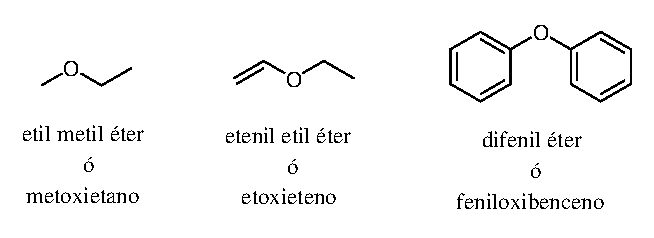
\includegraphics[scale=1]{eteres1.eps}
\end{figure}

\subsection{Aldehídos y Cetonas}

Son compuestos que poseen el grupo carbonilo \ch{-C=O} como grupo funcional.
\begin{enumerate}[label=\numberballmDarkTeal]
    \item \textbf{Aldehídos}: Grupo carbonilo en un átomo terminal y por lo tanto el carbono del grupo carbonilo se encuentro unido al menos a un átomo de hidrógeno.
          \begin{figure}[H]
              \centering
              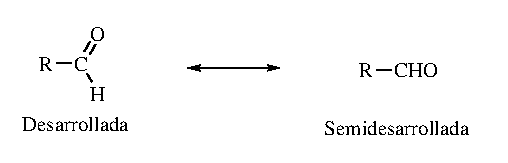
\includegraphics[scale=1]{aldehidos.eps}
          \end{figure}
    \item \textbf{Cetonas}: En las cetonas el grupo carbonilo \ch{-C=O} no se encuentra en un átomo terminal y por lo tanto el grupo carbonilo siempre estará unido a dos átomos de carbono. \ch{R-CO-R'}
          \begin{figure}[H]
              \centering
              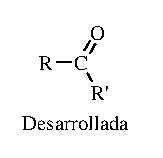
\includegraphics[scale=1]{cetona.eps}
          \end{figure}
\end{enumerate}

\mybox{Nomenclatura}

\begin{enumerate}[label=\numberballmDarkTeal]
    \item \textbf{Aldehídos}
          \begin{enumerate}
              \item Los aldehídos se nombran reemplazando la terminación \blueremark{-ano} del alcano correspondiente por \blueremark{-al}.
              \item No es necesario especificar la posición del aldehído puesto que ocupa siempre la posición terminal.
              \item El átomo de carbono donde se encuentra el grupo carbonilo, será el localizador 1.
              \item Si la molécula tiene dos grupos aldehído, se utiliza la terminación \blueremark{-dial}
              \item Si el grupo aldehído está en un ciclo se llama \blueremark{-carbaldehído}
                    \begin{figure}[H]
                        \centering
                        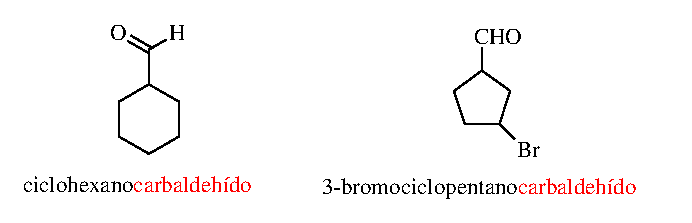
\includegraphics[scale=1]{adehido_2.eps}
                    \end{figure}
              \item Algunos nombres aceptados por la IUPAC de aldehídos son:
                    \begin{figure}[H]
                        \centering
                        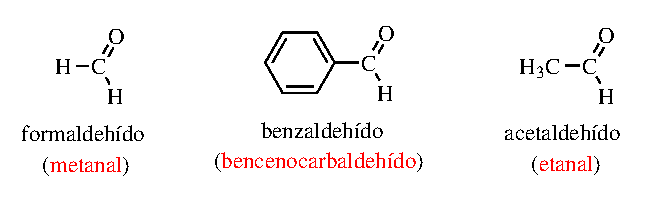
\includegraphics[scale=1]{adehido_3.eps}
                    \end{figure}
              \item Si la cadena principal presenta radicales, estos radicales se nombran antes de dicha cadena principal, luego el prefijo que indica el número de átomos de carbono de dicha cadena principal terminado en \blueremark{-al}. Si existiera alguna insaturación, su ubicación se señala anteponiendo el número localizador.
                    \begin{figure}[H]
                        \centering
                        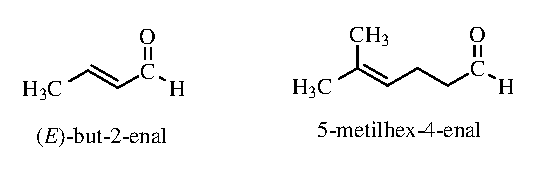
\includegraphics[scale=1]{adehido_4.eps}
                    \end{figure}
            \item Si actúa como radical, se utiliza el prefijo \blueremark{oxo-}.
          \end{enumerate}
    \item \textbf{Cetonas}
          \begin{enumerate}
              \item Las cetonas se nombran sustituyendo la terminación \blueremark{-ano} del alcano con igual longitud de cadena por \blueremark{-ona}.
              \item Se toma como cadena principal la de mayor longitud que contiene el grupo carbonilo.
              \item Se numera para que el grupo carbonilo tenga el localizador más bajo.
                    \begin{figure}[H]
                        \centering
                        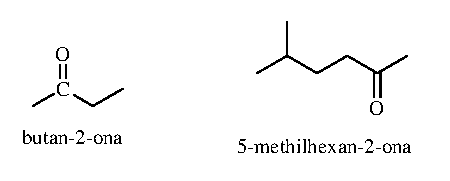
\includegraphics[scale=1]{cetona_2.eps}
                    \end{figure}
              \item Otra forma de nombrar las cetonas es nombrar las cadenas unidas al grupo carbonilo como sustituyentes, ordenarlas alfabéticamente y terminar el nombre con la palabra cetona.
                    \begin{figure}[H]
                        \centering
                        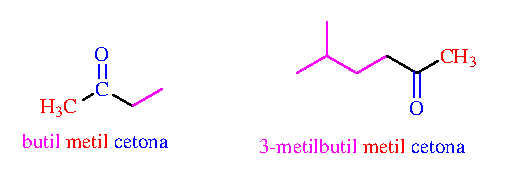
\includegraphics[scale=1]{cetona_3.eps}
                    \end{figure}
            \item Si actúa como radical, se utiliza el prefijo \blueremark{oxo-}
          \end{enumerate}
\end{enumerate}

\subsection{Ácidos Carboxílicos}

El grupo funcional del ácido carboxílico es:
\begin{figure}[H]
    \centering
    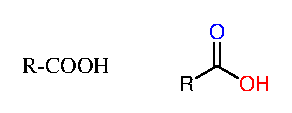
\includegraphics[scale=1]{acido1.eps}
\end{figure}

El grupo ácido carboxílico siempre se encuentra en posición terminal y se llama así porque pueden ceder fácilmente el hidrógeno que se encuentra unido al oxígeno dibujado en color rojo.\vspace{6pt}

\mybox{Nomenclatura}

\begin{enumerate}[label=\numberballmDarkTeal]
    \item Siempre se empieza con la palabra \blueremark{ácido} seguido del nombre del alcano del que procede añadiendo la terminación \blueremark{-ico}.
    \item Si hubiera dos o más grupos carboxílico se indicaría con la terminación \blueremark{-dioico}, \blueremark{-trioico} \dots.
    \item La cadena principal se empieza a numerar por el extremo donde se encuentre el grupo ácido.
    \item Si tenemos varios grupos ácidos, la cadena principal será aquella que genere los localizadores más bajos.
    \item Si tenemos dos grupos ácido y además insaturaciones, la cadena principal será aquella que genere el localizador más bajo a la insaturación.
    \item Si tenemos grupos ácidos con insaturaciones, se indican la posición de esa insaturación con localizadores usando al finar la terminación \blueremark{-enoico} para los dobles enlaces o \blueremark{-inoico} para los triples enlaces.
    \item Si tenemos más de dos dobles enlaces tendremos \blueremark{-dienoico}, \blueremark{-trienoico}.
\end{enumerate}

\begin{figure}[H]
    \centering
    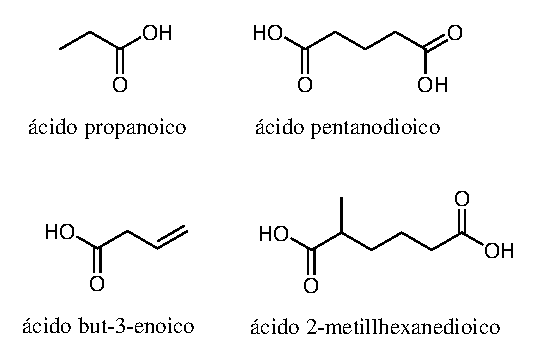
\includegraphics[scale=1]{acido2.eps}
\end{figure}

\subsection{Ésteres}

Los ésteres tienen el siguiente grupo funcional:

\begin{figure}[H]
    \centering
    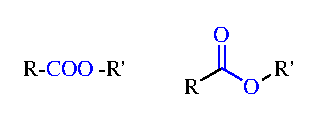
\includegraphics[scale=1]{esteres1.eps}
\end{figure}

\mybox{Nomenclatura}

\begin{enumerate}[label=\numberballmDarkTeal]
    \item Se identifican las dos cadenas R y R\(\prima{}\).
    \item La cadena principal será aquella que esté unida al grupo \ch{-C = 0}. Este grupo \ch{-C = 0} también debe contabilizarse para determinar la longitud de dicha cadena.
    % \item Se toma la cadena principal aquella de mayor longitud. El átomo de carbono del carbonilo (\ch{-C=0}) debe contarse para determinar la cadena
    \item Se nombran igual que los ácidos pero quitando la palabra ácido y cambiando la terminación \blueremark{-oico} por \blueremark{-oato} en la cadena principal seguido de la cadena secundaria nombrada como radical.
    \item Si tenemos sustituyentes en las cadenas, estas se empiezan a nombrar desde el carbono que está unido  al oxígeno (igual en ambas cadenas).
    \item Si tuviéramos alguna insaturación en las cadena principal estas se nombrarán indicando su localización con la terminación \blueremark{-enato}.
\end{enumerate}

\begin{figure}[H]
    \centering
    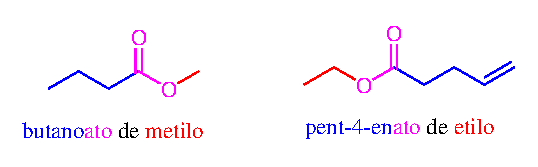
\includegraphics[scale=1]{esteres2.eps}
\end{figure}

\subsection{Aminas}

Se pueden considerar como los derivados del amoniaco \ch{NH3} ya que su obtención es mediante la sustitución de algunos de sus hidrógenos por sustituyentes orgánicos, normalmente alquilos o arilos. Su estructura final es \ch{-R_3N}.\vspace{6pt}

\mybox{Nomenclatura}:

\begin{enumerate}[label=\numberballmDarkTeal]
    \item Se nombran añadiendo como el alcano del que procede eliminando \blueremark{-o} y añadiendo \blueremark{amina}
    \begin{figure}[H]
        \centering
        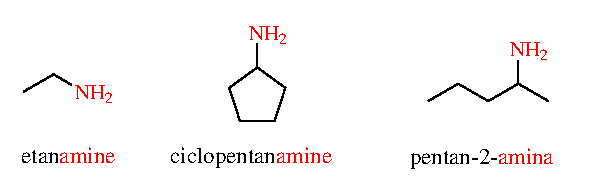
\includegraphics[scale=1]{amina1.eps}
    \end{figure}
        
    \item Si un radical está repetido varias veces se indican con los prefijos \blueremark{di-}, \blueremark{tri-} \dots Si tienen radicales diferentes se nombran por orden alfabético.
    \begin{figure}[H]
        \centering
        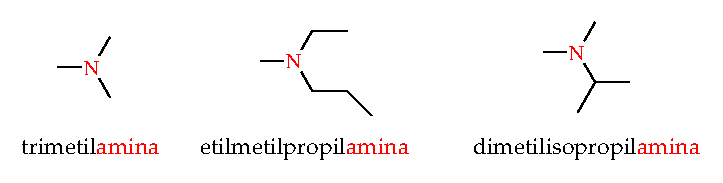
\includegraphics[scale=1]{amina2c.eps}
    \end{figure}

    \item Los radicales unidos  directamente al nitrógeno llevan el localizador \blueremark{N}. Si en la molécula hay dos grupos amino sustituidos se emplea \blueremark{N,N'}
          \begin{figure}[H]
              \centering
              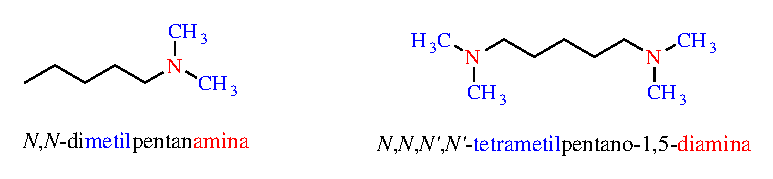
\includegraphics[scale=1]{amina3.eps}
          \end{figure}
\end{enumerate}

\subsection{Amidas}

Derivan de los ácidos carboxílicos (\ch{CO}\ch{OH}) al sustituir el grupo hidroxilo \ch{-OH} por grupos amino que dando por tanto su fórmula general de la siguiente manera: \ch{R}\azul{\ch{CO}}\rojo{\ch{NH2}} ó \ch{R}\azul{\ch{CO}}\rojo{\ch{NR'R''}}

\begin{figure}[H]
    \centering
    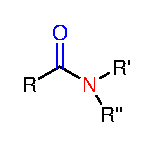
\includegraphics[scale=1]{amida1.eps}
\end{figure}

\mybox{Nomenclatura}

\begin{enumerate}[label=\numberballmDarkTeal]
    \item Se nombran como el alcano del que procede, hay que tener en cuenta que el carbono del grupo \ch{-C = 0} también se contabiliza para determinar el tamaño de la cadena. Se sustituye  \blueremark{-o} por \blueremark{-amida}
          \begin{figure}[H]
              \centering
              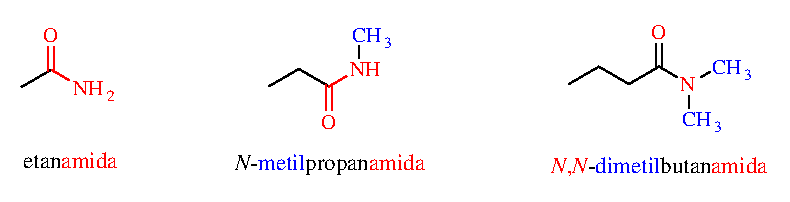
\includegraphics[scale=1]{amida4.eps}
          \end{figure}
    \item Si existen insaturaciones o cadenas laterales se indican con localizadores y la cadena empieza a numerarse por el extremo que tiene el grupo amido.
    \begin{figure}[H]
        \centering
        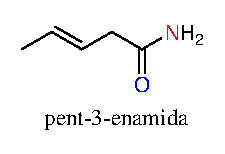
\includegraphics[scale=1]{amida2.eps}
    \end{figure}
    \item Si el nitrógeno del grupo amida contiene algún sustituyente, se específica este radical anteponiendo la letra \blueremark{N} y se escribe antes que el nombre de la amida.
    \begin{figure}[H]
        \centering
        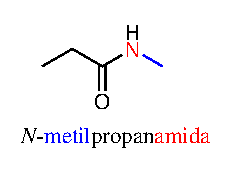
\includegraphics[scale=1]{amida3.eps}
    \end{figure}
    \item Cuando el grupo amida no es el grupo funcional y actúa como sustituyente se utiliza el prefijo \blueremark{carbamoil}.
          
    \item En compuestos cíclicos se nombra el ciclo y se termina con el sufijo \blueremark{-carboxamida}
    \begin{figure}[H]
        \centering
        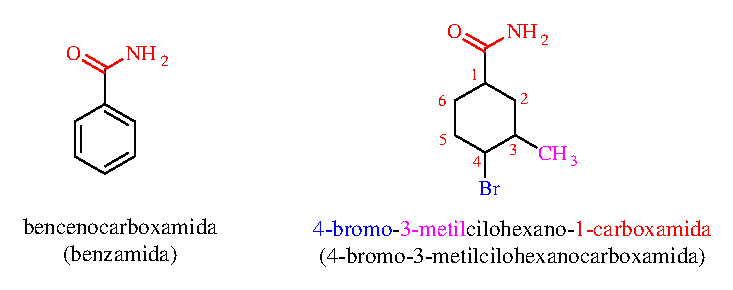
\includegraphics[scale=1]{amida5.eps}
    \end{figure}
          
\end{enumerate}

\section{Otros grupos de interés}

Otros grupos de interés son:

\subsection{Nitroderivados}

Son compuestos donde el grupo el grupo funcional es:

\begin{figure}[H]
    \centering
    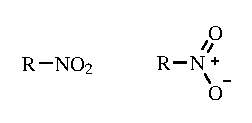
\includegraphics[scale=1]{nitro1.eps}
\end{figure}

\mybox{Formulación}\vspace{6pt}

Se nombran siempre como \textbf{sustituyente} con el prefijo \blueremark{nitro} y nunca como \textbf{cadena principal}

\begin{figure}[H]
    \centering
    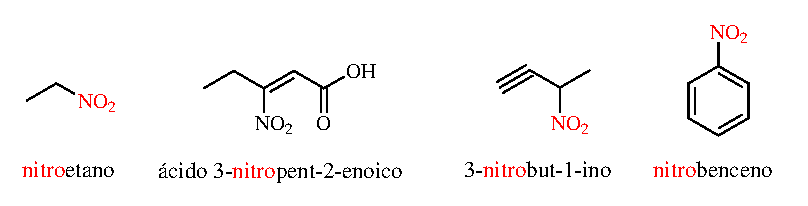
\includegraphics[scale=1]{nitro2.eps}
\end{figure}


\subsection{Nitrilos}

Su grupo funcional es:

\begin{figure}[H]
    \centering
    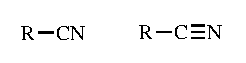
\includegraphics[scale=1]{nitrilo1.eps}
\end{figure}

\mybox{Nomenclatura}

\begin{enumerate}[label=\numberballmDarkTeal]
    \item Cuando actúa como grupo funcional se utiliza la terminación \blueremark{-nitrilo}
    \item Cuando actúa como radical se ula el prefijo \blueremark{ciano-}
\end{enumerate}

% \newpage{}

% \myemptypage{}

% \newpage{}



 \section{Ejercicios}



\subsection*{Alcanos}


\begin{enumerate}
    \item Formula los siguientes alcanos
          \begin{enumerate}
              \item n-pentano.
              \item 2,3,4-trimetilheptano.
              \item 4-etil-2,6-dimetiloctano.
              \item 4,6-dietil-2,4,8-trimetilnonano.
              \item 4-etil-2,2,5,8-tetrametil-6-propildecano.
              \item 3,7-dietil-5-isopripildecano.
          \end{enumerate}
    \item Nombra los siguientes alcanos
          \begin{enumerate}
              \item \chemfig{CH_3-CH(-[2]CH_3)-CH_2-CH(-[6]CH_3)-CH(-[2]CH_3)-CH_3}
              \item \chemfig{CH_3-CH(-[6]CH_3)-CH_2-C(-[2]CH_3)(-[6]CH_3)-CH_2-CH_2-CH_3}
              \item \chemfig{CH_3-CH(-[2]CH_3)-CH(-[6]CH_3)-CH_2-C(-[2]CH_3)(-[6]CH_3)-CH_3}
              \item \chemfig{CH_3-C(-[2]CH_3)(-[6]CH_3)-CH_2-CH(-[6]CH_2-CH_3)-CH([2]CH_3)-CH_2-CH(-[6]CH_3)-CH_3}
              \item \chemfig{CH_3-CH_2-CH(-[2]CH_3)-CH(-[6]CH_2-[6]CH_2-[6]CH_3)-CH(-[2]CH_3)-CH(-[6]CH_2-CH_3)-CH(-[2]CH_3)-CH_3}
              \item \chemfig{CH_3-CH_2-C(-[2]CH_3)(-[6]CH(-[4]CH_3)-[6]CH_3)-CH(-[6]CH_3)-CH(-[6]CH_2-CH_3)-CH_2-CH_2-CH_3}
          \end{enumerate}
\end{enumerate}

\subsection*{Alquenos}
\begin{enumerate}
    \item formula los siguientes alquenos
          \begin{enumerate}
              \item
              \item but-1-eno
              \item pent-2-eno
              \item hexa-2,4-dieno
              \item 3-butilhexa-1,4-dieno
              \item but-2-ino
              \item 3,4-dimetilpent-1-ino
              \item 3,6-dimetilnona-1,4,7-triino
              \item pent-1-en-3-ino
              \item hept-3-en-1,6-diino
              \item 4-etilhexa-1,3-dien-5-ino
          \end{enumerate}
    \item Nombra los siguientes alquenos
          \begin{enumerate}
              \item \chemfig{CH_3-CH=CH-CH_2-CH_2-CH_3}
              \item \chemfig{CH_3-CH_3-C(-[6]CH_3)=CH-CH_3}
              \item \chemfig{CH~C-CH(-[6]CH_3)-CH_2-CH_3}
              \item \chemfig{CH_3-CH=C(-[6]CH_3)-CH_2-CH_3}
              \item \chemfig{CH~C-C~C-CH_2-CH_3}
              \item \chemfig{CH~C-CH=CH-CH_3}
              \item \chemfig{CH_2=CH-C(-[6]CH_3)-CH_2-CH_2-C~CH}
              \item \chemfig{CH_3-CH=C(-[6]CH_3)-CH_2-C~C-CH(-[2]CH_3)-CH=CH_2}
              \item \chemfig{CH_2=CH-CH(-[6]CH(-[6]CH_3)-CH_3)-CH_2-C~C-CH(-[6]CH_2-[6]CH_3)-C~CH}
          \end{enumerate}
\end{enumerate}

\subsection*{Hidrocarburos cíclicos}

\begin{enumerate}
    \item Formula los siguientes hidrocarburos cíclicos:
          \begin{enumerate}
              \item Etilciclohexano
              \item Ciclopenteno.
              \item Ciclohexino
              \item 1,1,4,4-tetrametilciclochexano
              \item 3-etilciclopenteno
              \item 2,3-dimetilciclohexeno
              \item 4-ciclobutilpent-1-ino
              \item 3-ciclohexil-5-metilhex-2-enociclohexa-1,3-dieno
              \item 3-ciclopentilprop-1-eno
          \end{enumerate}
    \item Nombra los siguientes hidrocarburos
          \begin{enumerate}
              \item \chemfig{*4(----)}
              \item \chemfig{*6(-----=)}
              \item \chemfig{*6(---(-CH_3)--(-CH_2-[2]CH_3)-)}
              \item \chemfig{*6(---=-=)}
              \item \chemfig{*6(---(-CH(-[:50]CH_3)(-[:-50]CH_3))---)}
              \item \chemfig{CH_3-CH(-[6]*6(------))-CH_2-CH_2-C(-[2]CH_3)(-[6]CH_3)-CH_2-CH_3}
              \item  \chemfig{CH_3-CH(-[6]*5(-----))-CH=CH_2}
          \end{enumerate}
\end{enumerate}

\subsection*{Hidrocarburos aromáticos}
\begin{enumerate}
    \item Formula los siguientes hidrocaruros aromáticos:
          \begin{enumerate}
              \item Metilbenceno (tolueno)
              \item 1,3-dietilbenceno
              \item Etenilbenceno
              \item 1-butilñ4-isopropilbenceno
              \item \textit{p-}propiltolueno
              \item 3-fenil-5-metilheptano
              \item 4-fenilpent-1-eno
              \item 2,4-difenil-3-metilhexano
          \end{enumerate}
    \item Nombra los siguientes hidrocarburos aromáticos
          \begin{enumerate}
              \item \chemfig{**6(----(-CH(-[:180]H_3C)([:0]-CH_2-C(-[2]CH_3)(-[6]CH_3)(-CH_3)))--)}
              \item \chemfig{**6(----(-CH_2-[:0]CH_3)--)}
              \item \chemfig{**6(-(-CH_2-[:0]CH_2-[0]CH_3)--(-CH_3)---)}
              \item \chemfig{**6(-(-CH_3)--(-CH_3)--(-CH_3)-)}
              \item \chemfig{**6(----(-CH(-[1]CH_3)(-[3]H_3C))--)}
              \item \chemfig{**6(--(-[:0]CH_2-[:0]CH_2-[:0]CH_2(-[:0]**6(------)))----)}
              \item \chemfig{CH_3-CH=C(-[6]**6(------))-CH_2-CH_3}
          \end{enumerate}
\end{enumerate}
\subsection{Derivados halogenados}
\begin{enumerate}
    \item Formula los siguientes derivados halogenados
          \begin{enumerate}
              \item 2-cloropropano
              \item 1,3-dibromobenceno
              \item 1,1,2,2-tetrafluoretano
              \item 1,4-diclorociclohexano
              \item 4-bromopent-1-ino
              \item 3-fluor-5-metilhex-2-eno
              \item 1,4-dibromo-6-ciclopentiloct-2-eno
              \item 4-yodo-2,5-difenilpent-1-ino
              \item 4-clorobut-1-eno
              \item 1,2-dibromobenceno
          \end{enumerate}
    \item Nombra los siguientes derivados halogenados
          \begin{enumerate}
              \item \chemfig{CH_3-I}
              \item \chemfig{CH_2(-[2]Cl)-CH_2(-[6]Cl)}
              \item \chemfig{CH_3-C(-[2]Br)(-[6]Br)-CH_2-CH_3}
              \item \chemfig{CH_2(-[2]Cl)-CH_2-CH=CH_2}
              \item \chemfig{CH~C-CH(-[2]Br)-CH_2-CH_2-Br}
              \item \chemfig{**6(----(-F)--)}
              \item \chemfig{CH_3-CH(-[2]Cl)-CH_2-CH_2(-*4(----))}
              \item \chemfig{*6(-(-Br)--(-Br)---)}
              \item \chemfig{CH_2(-[4]F)-CH(-[2]F)(-[6]F)}
              \item \chemfig{*5(-(-Cl)---(-Cl)-)}
          \end{enumerate}
\end{enumerate}
\subsection*{Alcoholes y éteres}
\begin{enumerate}
    \item Formula los siguientes alcoholes y éteres:
          \begin{enumerate}
              \item 3-metilpentan-1-ol.
              \item Butano-1,2,3-triol.
              \item 2-fenilpropano-1,3-diol.
              \item ciclohexanol.
              \item Hexa-3,5-dien-2-ol.
              \item Fenol (Hidroxibenceno).
              \item 2-etil-pentan-1-ol.
              \item Pent-3-en-1-ol.
              \item Etilisopropiléter.
              \item Etenilfeniléter.
              \item Dimetiléter.
              \item Butilciclopentiléter.
          \end{enumerate}
    \item Nombra los siguientes alcoholes y éteres.
          \begin{enumerate}
              \item \chemfig{CH_3-OH}
              \item  \chemfig{CH_2(-[2]OH)-CH_2-CH(-[6]CH_2-CH_3)-CH=CH_2}
              \item  \chemfig{CH_3-CH(-[2]OH)-CH(-[6]Br)-CH_2(-[2]OH)}
              \item \chemfig{CH_3-CH_2-CH(-[3]CH_3)-CH(-[6]CH_3)-CH(-[2]OH)=CH_2}
              \item \chemfig{CH_2=CH-CH(-[2]OH)-CH_2(-OH)}
              \item \chemfig{CH_3-CH_2-CH_3-O-CH_2-CH_2-CH_3}
              \item \chemfig{CH_2=CH-O-CH(-[2]CH_3)-CH_3}
              \item \chemfig{CH_3-CH_2-CH_2-CH_2-CH_2-O-C~H}
          \end{enumerate}
\end{enumerate}
\subsection*{Aldehídos y cetonas}
\begin{enumerate}
    \item Formula los siguientes aldehídos y cetonas.
          \begin{enumerate}
              \item Etanal (acetaldehído.)
              \item 3-metilpentanal
              \item Propenal.
              \item 5-ciclohexilpent-3-inal.
              \item Hex-2-endial.
              \item Hexa-2,4-diona.
              \item 1,4-difenilpentan-2-ona.
              \item Benzaldehído.
              \item 2-metilpentanodial.
              \item Hex-2-endial3-metilpent-2-enal.
              \item Pentan-2-ona.
              \item 3-clorobutanona.
              \item hexa-1,5-dien-3-ona.
          \end{enumerate}
    \item Nombra los siguientes aldehídos y cetonas.
          \begin{enumerate}
              \item \chemfig{H-!{aldehido}}
              \item \chemfig{CH_3-CH_2-CH_2-!{aldehido}}
              \item \chemfig{!{aldehido2}-CH=CH-!{aldehido}}
              \item \chemfig{CH_2=CH(-[:270]**6(------))-CH-CH-!{aldehido}}
              \item \chemfig{!{aldehido2}-CH=CH-CH_2-CH(-[2]CH_3)-!{aldehido}}
              \item \chemfig{CH_3-CH(-[6]!{fenil})-CH=CH-!{aldehido}}
              \item \chemfig{!{aldehido2}-CH_2-C~C-CH_2-CH_2-!{aldehido}}
              \item \chemfig{CH_3-C(=[2]O)-CH_2-CH_3}
              \item \chemfig{CH_3-CH=CH-CH_2-C(=[2]O)-CH_3}
              \item \chemfig{CH_3-C(=[2]O)-CH_2-CH_2-CH_2-C(=[2]O)-CH_3}
              \item \chemfig{CH_3-CH(-[2]CH_3)-C(=[6]O)-CH_2-CH(-[2]CH_3)-CH_3}
              \item \chemfig{CH_2=CH-C(=[2]O)-CH=CH-CH_3}
          \end{enumerate}
\end{enumerate}

\subsection*{Ácidos y Ésteres}

\begin{enumerate}
    \item Formula los siguientes ácidos y ésteres:
          \begin{enumerate}
              \item ácido etanoico (ácido acético)
              \item ácido 3-metilhexanoico
              \item ácido 2-feilpentanodioico
              \item ácido tricoloroetanoico
              \item ácido but-3-enoicoácido hepta-2,4-dienoicoácido pent-2-enodioico
              \item ácido benzoico
              \item butanoato de metilhexanopropanoato de tiolbenzoato de propiltoluenoetanoato de octilo
              \item 3-cloropentanoato de Etenilbencenobut-3-enoato de isopropilo
          \end{enumerate}
    \item Nombra los siguientes ácidos y ésteres:
          \begin{enumerate}
              \item \chemfig{CH_3-CH_2-CH_2-!{acido}}
              \item \chemfig{!{acido2}-CH_2-CH_2-!{acido}}
              \item \chemfig{CH_3-CH=CH-CH_2-!{acido}}
              \item \chemfig{CH_2-CH(-[2]CH_3)-CH_2-CH(-[2]CH_3)-CH_2-!{acido}}
              \item \chemfig{!{acido2}-C~C-CH_2-!{acido}}
              \item \chemfig{CH_3-CH_3-CH(-[6]!{ciclopentil})-!{acido}}
              \item \chemfig{CH_3-C(=[2]O)(-O-CH_3)}
              \item \chemfig{CH_3-CH_2-CH_2-C(=[2]O)(-O-CH_2-CH_3)}
              \item \chemfig{CH_3-CH_2-CH_2-CH_2-CH_2-CH_2-CH_2-C(=[2]O)(-O-CH_2-CH_2-CH_3)}
              \item \chemfig{CH_3-CH_2-CH_2-CH_2-CH_2-C(=[2]O)(-O-CH_3)}
              \item \chemfig{CH_3-CH(-[2]Br)-CH_2-C(=[2]O)(-O-CH=CH_2)}
              \item \chemfig{CH_2(-[:180]!{fenil})-CH_2-C(=[2]O)(-O-CH_2-CH_2-CH_2-CH_2-CH_2-CH_3)}
          \end{enumerate}
\end{enumerate}


\section{Compuestos Nitrogenados}

\begin{enumerate}
    \item Formula los siguientes compuestos nitrogenados:
          \begin{enumerate}
              \item isopropilamina
              \item penta-3-aminabuta-1,3-diamina
              \item 3-etil-diamina.
              \item 3-etilhexan-3-amina3,5-dimetilhexan-1-amina
              \item 3,5-dimetilhexan-1-amina
              \item pent-3-en-2-amina
              \item pent-3-en-2-amina
              \item N-metilfenilamina
              \item N-cilopentilbutilamina
              \item Etanamida
              \item N-metilietanamida
              \item 4-fenilpentamida
              \item N-etilhexa-4-enamida
          \end{enumerate}
    \item Nombra los siguientes compuestos nitrogenados
          \begin{enumerate}
              \item \chemfig{CH3-CH(-[6]NH_2)-CH2-CH3}
              \item \chemfig{CH_3-CH2-CH2-NH_2}
              \item \chemfig{CH3-CH(-[6]NH_2)-CH3-CH(-[6]NH_2)-CH2-CH2-NH_2}
              \item \chemfig{CH3-CH(-[6]CH3)-NH-CH=CH2}
              \item \chemfig{CH3-CH2-CH2-CH2-CH2-C(=[2]O)(-NH_2)}
              \item \chemfig{CH3-CH2-CH2-CH2-CH2-C(=[2]O)(-NH_2)}
              \item \chemfig{CH3-CH=CH-CH2-C(=[2]O)(-NH_2)}
              \item \chemfig{CH3-CH2-CH(-[2]Br)-CH2-CH2-C(=[2]O)(-NH-CH3)}
          \end{enumerate}
\end{enumerate}


\end{document}
